\subsection{Filter}
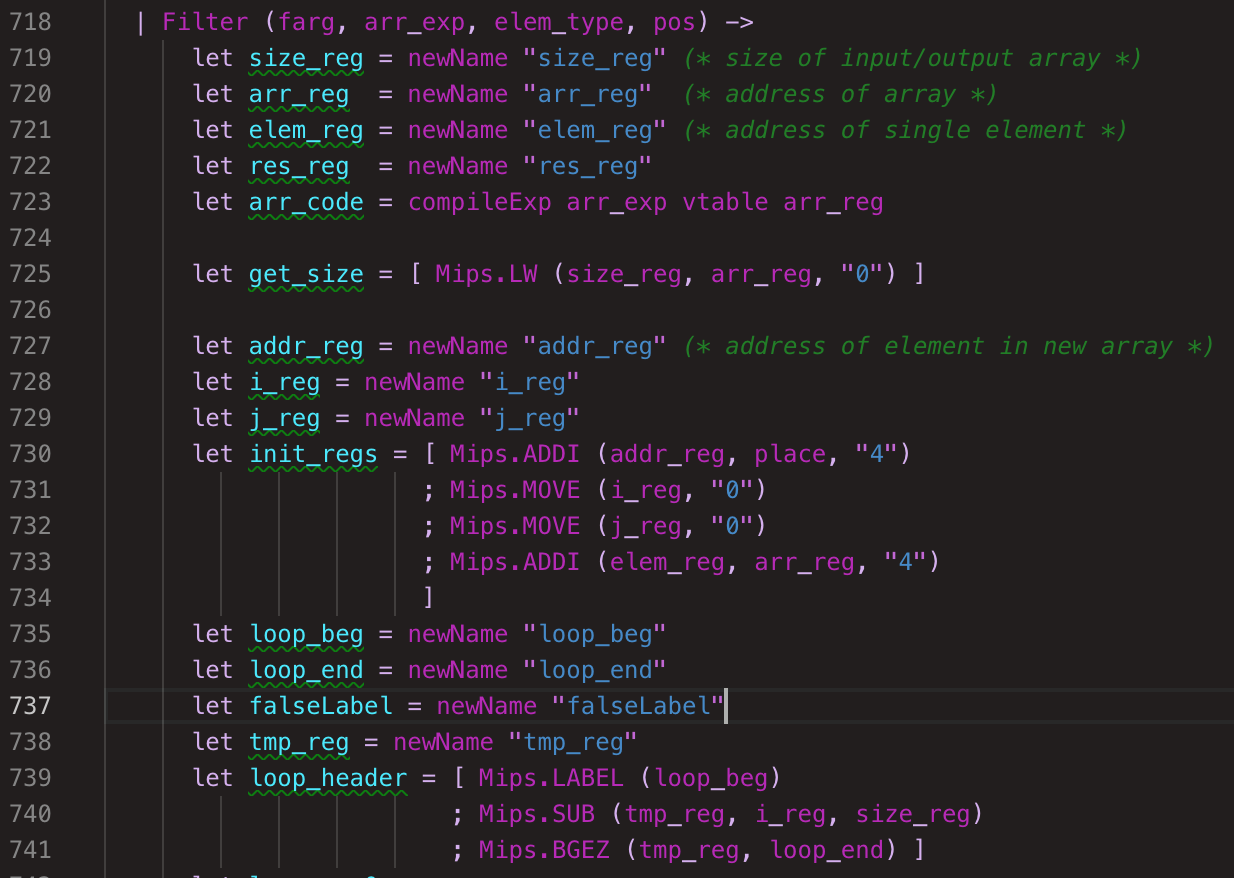
\includegraphics[width=\linewidth]{Materials/CodeGen/filterIntro}
Filter is implemented much like 'map'. To implement filter we first create a new array of the same size as the input array. We also create some new registers to keep track of the memory locations of the elements in the new array (\textit{addr\_reg}) and the input array (\textit{elem\_reg}). Lastly we create a register (\textit{j\_reg}) to count how many elements we have added to the new array.\\
The idea is we create a loop where we apply the input function on the first element of the input array, and if the output is \textit{true} we then add it to the new array, we add to the registers working as pointers to the elements in the array such that we move to the next entry in the arrays and lastly we add one to our counter register \textit{j\_reg}. If the output is \textit{false}, we only add to the \textit{elem\_reg} and then begin the loop anew on the next element of the input array.\\
We do this by loading the value of the input array into \textit{res\_reg} and apply the input function using the helper function \textit{applyFunArg} on lines 751-756.
 
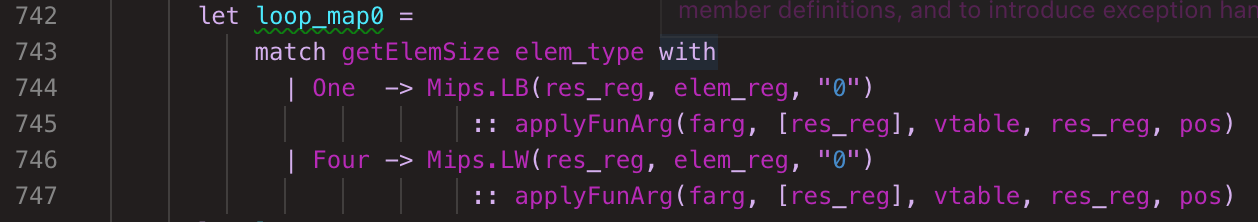
\includegraphics[width=\linewidth]{Materials/CodeGen/filter1}
We now have either '1' or '0' (true, false) in \textit{res\_reg}. We now load the value of \textit{elem\_reg} into a temporary register for use if the result is true. Then we add to \textit{elem\_reg} to have it point to the next entry of the input array. We now do a conditional branching. If the value of \textit{res\_reg} is true, we fall through, else we jump. In the case the result is \textit{true}, we save the value in \textit{tmp\_reg} in \textit{addr\_reg}, we add to \textit{addr\_reg} such that it points to the next entry of the array and we add 1 to \textit{j\_reg}. Then we meet the point where we would jump to if the result had been false (line 771), and the loop begins anew. All of this is done on lines 757-773. When the loop terminates after having iterated over all entries in the input array, we then shrink the size of our new array to its actual size using \textit{j\_reg} on line 775.

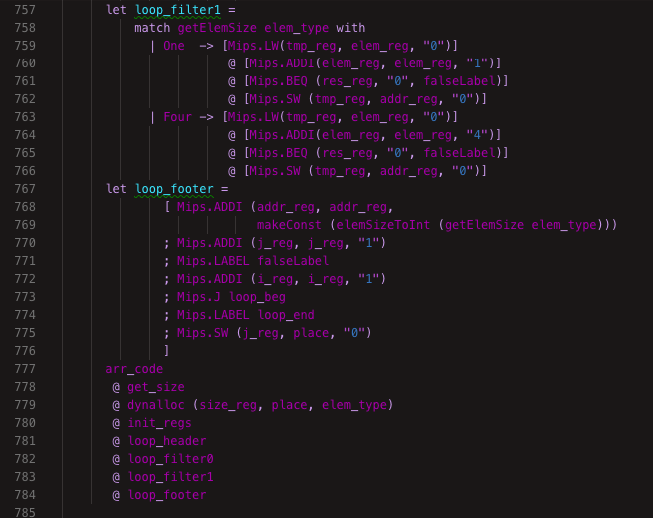
\includegraphics[width=\linewidth]{Materials/CodeGen/filter2}